\section{Speed Reading}
Speed reading is the act of trying to read faster than normal. There are various ways to read a given text, depending on the context and the purpose of the reading \cite{differentWaysOfReading}. A study has shown than when reading on paper, people read an average of 201 words per minute (WPM) and about 180 WPM when reading on a monitor (depending on its resolution) \cite{ziefle_effects_1998}. Speed reading is all about raising one's words per minute. Numerous techniques have been utilized throughout the years, and  thanks to computers reading software is becoming more available these days.


\subsection{Rapid Serial Visual Presentation (RSVP)}
Rapid Serial Visual Presentation is a technique that has become popular in the few last years. It's the idea of presenting words in small flashes, one at a time. In traditional reading, jumping from one word to another is done by saccading, which has a time penalty, since the eyes physically have to move back and forth. In RSVP, the goal is to eliminate saccading, thereby increasing reading speed. One of the more popular RSVP solutions is Spritz. According to their website, about 80\% of the time spent reading is used on physically moving the eyes from word to word \cite{spritz}.	It is claimed that by utilizing RSVP, it is possible to reduce this time. Additionally, by aligning the words according to the optimal recognition position (see Section \ref{ORP}), results can get even faster. Figure \ref{fig:spritz_orp} illustrates this concept.

\begin{figure}[htbp]
\centering
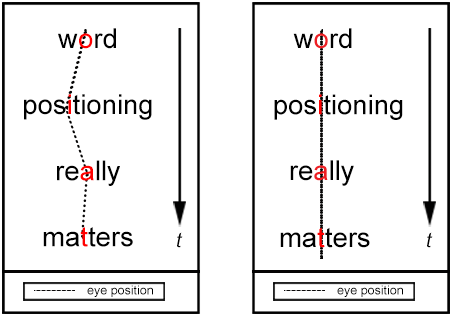
\includegraphics[width=0.3\textwidth]{Pics/opr_spritz}
\caption{Spritz utilizes the optimal recognition position to align words.}
\label{fig:spritz_orp}
\end{figure}


Explaining what is it
Spritz example
Critique of RSVP - Add critique points on the fly (ALL!)
Summary of Don't Believe What You Read (Only Once): Comprehension Is Supported by Regressions During Reading

\subsection{Critiques of Speed Reading}
In order to test how efficient RSVP actually is, a study from 2014 was conducted by Schotter, Tran \& Rayner \cite{schotter_dont_2014}. One thing that is criticized with RSVP techniques is the ability to go back and re-read words for improving one's comprehension. This process is called \textit{regression}, and according to \cite{schotter_dont_2014} about 10\% to 15\% of time spent reading is by making regressions, i.e. moving eyes back in the text to read material that has previously been processed. The hypothesis is that regression supports reading comprehension, since it allows readers to access more information from the text. This is especially true with texts that are more difficult to read, i.e. that it requires the reader to go back and read words again to make sense of how the sentence is structured. Readers are more likely to make a regression when they sense that their comprehension of the sentence has faltered \cite{schotter_dont_2014}.

You can't regress - Loss of comprehension
Loss of spatial awareness and formatting
